\subsection{Arquitectura global}

\begin{figure}[H]
\centerline{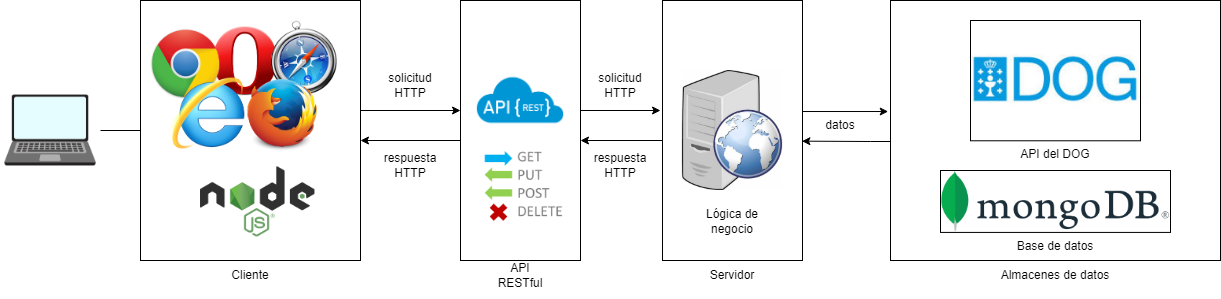
\includegraphics[width=15cm]{figuras/diseño/arquitecturaglobal.PNG}}
\caption{Arquitectura global del sistema.}
\label{enlaceArquitecturaGlobal}
\end{figure}

En esta aplicación se utiliza una arquitectura basada en servicios REST \cite{rest}. Este tipo de arquitecturas se caracterizan por el acceso a recursos de forma simple mediante solicitudes HTTP, además de permitir un desacople entre interfaz y servidor. La arquitectura del sistema es ilustrada en la \hyperref[enlaceArquitecturaGlobal]{Figura 3.1}.
\\

El cliente está conformado por todos aquellos navegadores web que realizan llamadas a la API del servidor mediante su propia interfaz. El usuario accede a cualquier navegador y puede utilizar la aplicación. De todas formas, existen algunos clientes web donde la aplicación no es soportada debido a que se utilizan las últimas características de JavaScript. Es por ello que para poder utilizar esta aplicación se han de utilizar navegadores evergreen \cite{evergreen} (que se actualizan automáticamente a sus futuras versiones).
\\

Desde el cliente se realizan solicitudes HTTP hacia la API RESTful, que expone todos los servicios implementados en el servidor. Gracias al uso de la arquitecutra REST, se permite el acceso a los recursos mediante URIs, las cuales pueden ser accedidas mediante los verbos HTTP (GET para obtener información, POST para crear objetos, PATCH y PUT para modificar información, y DELETE para eliminar objetos). Al cliente se le devuelve desde la API una respuesta HTTP con todas sus cabeceras. Y, además, en el caso de las operaciones GET, POST, PATCH y PUT, además, se devuelve el objeto correspondiente a la operación, ya se haya obtenido, creado o modificado.
\\

La API, como se ha mencionado anteriormente, expone los servicios del servidor. En el servidor es donde se aplica la lógica de negocio \cite{logicanegocio} de la aplicación, es decir, donde se crea, almacena y modifica la información.
\\

En cuanto a la información que se utiliza en la aplicación, esta puede ser obtenido de dos fuentes diferentes. Por un lado, se obtiene información del DOG a través de su API REST, la cual se corresponde con las leyes que todavía no están almacenadas en la base de datos de la aplicación. El otro método para obtener información es directamente de la base de datos de MongoDB \cite{mongodb}, donde se encuentran las leyes consolidadas.
\\

En cuanto a la base de datos empleada (MongoDB), cabe mencionar que esta es una base de datos NoSQL \cite{nosql}. Este tipo de bases de datos se caracterizan por estar orientadas hacia documentos, y almacenan y recuperan los datos en formatos que no son tablas.
\\

Con esta arquitectura se ha logrado el cumplimiento de dos requisitos no funcionales descritos: el {\bf NFR-08: Uso de tecnologías web y servicios RESTful} y el {\bf NFR-09: Base de datos NoSQL}.